 \section{Propuesta}
\subsection{Requerimientos}
\begin{frame}{Propuesta de solución}
	\begin{block}{El desarrollador requiere}
		\begin{itemize}
		  \item Definir políticas de seguridad desde la implementación de sus aplicativos.
		  \item Una herramienta que verifique las políticas definidas.
		  \item Garantizarle al usuario que la aplicación respeta determinadas
		  políticas de seguridad.
		\end{itemize}
	\end{block}
\end{frame}

\subsection{Propuesta}
\begin{frame}{Propuesta de solución}
	\begin{block}{Propuesta}
		  Proveer una herramienta de análisis de flujo de información mediante el
		  sistema de anotaciones de Jif.
	\end{block}
	\center{Herramienta de Análisis Estático}
	\begin{figure}[t!]
		\begin{center} 
		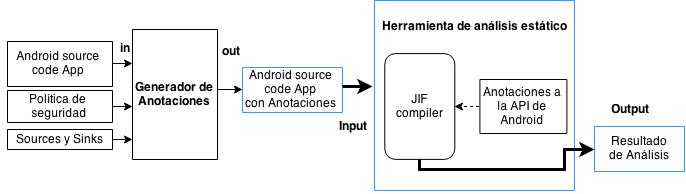
\includegraphics[width=9cm]{desing3Real-2-2-azul.jpg} 
		\end{center}
	\end{figure}
\end{frame}

\subsection{Jif}
\begin{frame}{Características de Jif}
\begin{itemize}
  \item Lenguaje tipado de seguridad.
  \item Extensiones de seguridad al lenguaje java.
  \item Restricciones para uso de la información.
  \item Análisis de flujo de información mediante chequeo de etiquetas.
\end{itemize}
\end{frame}
\begin{frame}[fragile]{Características sobresalientes de Jif}
\begin{columns}[T]
\column{2in}
	\begin{itemize}
	  \item Anotar propiedades de seguridad.
	  \item Verificar las propiedades de seguridad.
	  \item Cubrir todas las posibles ramas de ejecución en el análisis.
	  \item Diseñado para aplicativos Java.
	\end{itemize}
\column{2in}{Flujos explícitos - Flujos implícitos}
	

\end{columns}
\end{frame}

\subsection{Propuesta - especificaciones}
\begin{frame}{}

\end{frame}


















\begin{frame}{Política de Seguridad}
	\begin{columns}[c]
	\column{1.5in}
	\begin{center}
	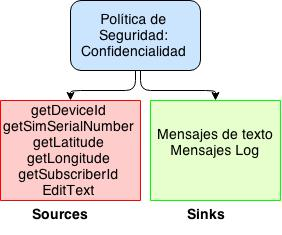
\includegraphics[width=5cm]{Politica.jpg} 
	\end{center}
	\column{1.5in}
	Flujos de información entre: información con nivel de seguridad alto(sources) e
	información con nivel de seguridad bajo(sinks).
	\end{columns}
\end{frame}

\subsection{Lineamientos de Anotación} 
\begin{frame}{Autoridad y Labels de Anotación}
	\center{Autoridad Máxima}
	\begin{center}
	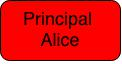
\includegraphics[width=2cm]{Principal.jpg}
	\end{center}
	\begin{columns}[T]
	\column{2in}
	Nivel de Seguridad Alto:
	\begin{center}
	\vspace{-0.5em}
	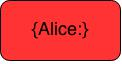
\includegraphics[width=2cm]{high.jpg}\newline
	\vspace{-1.5em}
	\end{center}
	Sólo el principal \emph{Alice}\\ dueño de la política \\ podrá leer la
	información.
	\column{2in}
	Nivel de Seguridad Bajo:
	\begin{center}
	\vspace{-0.5em} 
	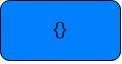
\includegraphics[width=2cm]{low.jpg}\newline
	\vspace{-1.5em}
	\end{center}
	No se define un principal,\\
	todos pueden leer\\
	la información.
	\end{columns}
\end{frame}	
\begin{frame}{Anotaciones a la API} %Anotaciones para
	\begin{block}{Controlar canales} 
	\begin{itemize}
	  \item Mensajes de texto (SmsManager)
	  \item Mensajes log (Log)
	\end{itemize} 
	\end{block}
	\pause
	\begin{block}{Clases adicionales requeridas}
		\begin{itemize}
		  \item Clases para los sources (TelephonyManager)
		  \item Clases para métodos de sobresscritura (Activity)
		\end{itemize}
	\end{block}
\end{frame}	
\begin{frame}[fragile]{Anotaciones a la API}
\begin{block}{Controlar canales}
\begin{lstlisting}[style=base]
<sendTextMessage>@{Alice:}@ <(> 
String@{Alice:}@ destinationAddress, 
String@{Alice:}@ sourceAddress, 
String-{}-text, 
PendingIntent@{Alice:}@ sentIntent,
PendingIntent@{Alice:}@ deliveryIntent 
<)>{}
\end{lstlisting} 
\end{block}
\end{frame}
% \begin{frame}{Clases adicionales requeridas}
% 	\begin{block}{Mecanismos}
% 		\begin{itemize}
% 		  \item Anotación
% 		  \item Signaturas Nativas
% 		  \item signaturas nativas más labels de Seguridad
% 		\end{itemize}
% 	\end{block}
% \end{frame}

\begin{frame}{Anotaciones a la API}
	\begin{figure}[t!]
		\begin{center} 
		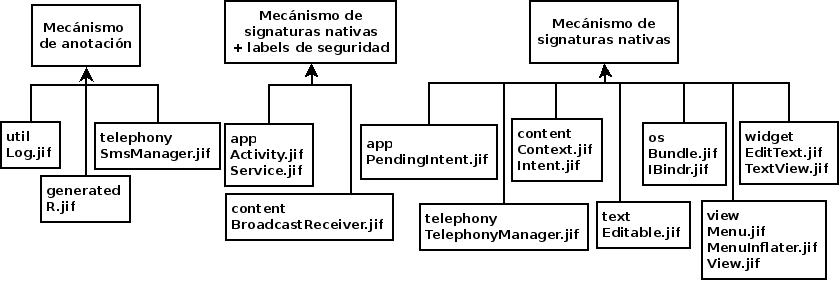
\includegraphics[width=9cm]{annotationsMechanims.jpeg} 
		\end{center}
	\end{figure}
\end{frame}
\begin{frame}{Anotación de aplicativos a analizar}
	\begin{columns}[c]
		\column{1.5in}{Generador de Anotaciones}
			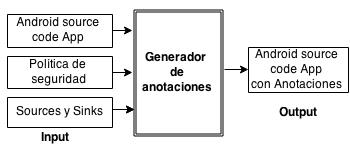
\includegraphics[width=4cm]{desingSolution2-2.jpg}
		\column{1.5in}
			\begin{itemize}
	  		\item Objetivo de la anotación
	  		\item Elementos a anotar
			\end{itemize}
	\end{columns}
\end{frame}
% \begin{frame}{Anotación de aplicativos a analizar}
% 	\begin{lstlisting}[style=base]
% 	TelephonyManager {Alice:}mgr = (TelephonyManager) context.getSystemService(Context.TELEPHONY_SERVICE);
%     SmsManager sms = SmsManager.getDefault();
%     sms.sendTextMessage("+49 1234", null, mgr.getDeviceId(), null, null);
% 	\end{lstlisting}
% \end{frame}